%!TEX root =../mapp-challenge-18-game-book.tex
% ^ leave for LaTeXTools build functionality

\phChapterWorksheet{Go For It!}{Main Puzzle 1}

While traveling down Road \(4.139\pi\),
you cross paths with a wizened \mappMobidot{} Trainer. After finally
completing his
\textbf{non-skippable seven-hour tutorial} on how to catch \mappMobimon{},
you try to slip away without him noticing. Alas, before you can make your
excuses, he begins to tell you how \mappMobidot{} battles were fought
\textbf{back in his day}.

Before \mappMobimon{} battles were limited to one-on-one matches,
two trainers would send all their \mappMobidot{} into battle at once. Trainers
would often practice battling by \textbf{alternatively placing
black and white stones} on the intersections of lines on a grid,
representing the positions of each trainer's \mappMobimon{}. The old man,
not bothering to hide his frustration that you aren't showing any
interest in this bit of history, insists on showing you the following example.

\begin{center}
  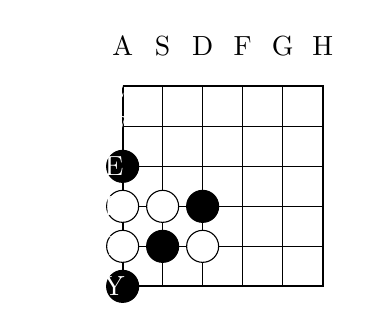
\begin{tikzpicture}[x=0.2in,y=0.2in]
    \draw[step=1] (0,0) grid (5,5);
    \draw[thick] (0,0) rectangle (5,5);
    \draw[fill=white] (0,1) circle (0.4);
    \draw[fill=white] (0,2) circle (0.4);
    \draw[fill=white] (1,2) circle (0.4);
    \draw[fill=white] (2,1) circle (0.4);
    \draw[fill=black] (0,0) circle (0.4);
    \draw[fill=black] (1,1) circle (0.4);
    \draw[fill=black] (2,2) circle (0.4);
    \draw[fill=black] (0,3) circle (0.4);
    \node at (-1,0) {\textcolor{white}{\contour{black}{Y}}};
    \node at (-1,1) {\textcolor{white}{\contour{black}{T}}};
    \node at (-1,2) {\textcolor{white}{\contour{black}{R}}};
    \node at (-1,3) {\textcolor{white}{\contour{black}{E}}};
    \node at (-1,4) {\textcolor{white}{\contour{black}{W}}};
    \node at (-1,5) {\textcolor{white}{\contour{black}{Q}}};
    \node at (0,6) {A};
    \node at (1,6) {S};
    \node at (2,6) {D};
    \node at (3,6) {F};
    \node at (4,6) {G};
    \node at (5,6) {H};
  \end{tikzpicture}
\end{center}

The senile old coot explains that a \textbf{group} of stones is formed when
the stones are positioned directly adjacent horizontally
or vertically on the board. A group of stones (or a single stone) will
be defeated if they are \textbf{completely surrounded by a group of
opposite-colored stones} vertically and horizontally, as in the following
example.

\begin{center}
  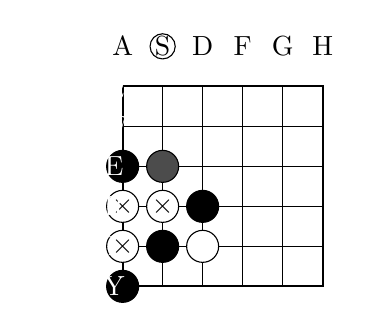
\begin{tikzpicture}[x=0.2in,y=0.2in]
    \draw[step=1] (0,0) grid (5,5);
    \draw[thick] (0,0) rectangle (5,5);
    \draw[fill=white] (0,1) circle (0.4);
    \draw[fill=white] (0,2) circle (0.4);
    \draw[fill=white] (1,2) circle (0.4);
    \draw[fill=white] (2,1) circle (0.4);
    \draw[fill=black] (0,0) circle (0.4);
    \draw[fill=black] (1,1) circle (0.4);
    \draw[fill=black] (2,2) circle (0.4);
    \draw[fill=black] (0,3) circle (0.4);
    \draw[fill=black!70] (1,3) circle (0.4);
    \node at (0,1) {\(\times\)};
    \node at (0,2) {\(\times\)};
    \node at (1,2) {\(\times\)};
    \node at (-1,0) {\textcolor{white}{\contour{black}{Y}}};
    \node at (-1,1) {\textcolor{white}{\contour{black}{T}}};
    \node at (-1,2) {\textcolor{white}{\contour{black}{R}}};
    \node at (-1,3) {\textcolor{white}{\contour{black}{E}}};
    \node at (-1,4) {\textcolor{white}{\contour{black}{W}}};
    \node at (-1,5) {\textcolor{white}{\contour{black}{Q}}};
    \node at (0,6) {A};
    \node[draw,circle,inner sep=0.1pt] at (1,6) {S};
    \node at (2,6) {D};
    \node at (3,6) {F};
    \node at (4,6) {G};
    \node at (5,6) {H};
  \end{tikzpicture}
\end{center}

You haven't really been listening, but then the old man mentions that he
might be able to tell you where to \textbf{find some interesting Plant-type
\mappMobimon{}} if you can solve this \textbf{puzzle}.
In each of the provided \textbf{Old-School \mappMobimon{} Battle Grids},
there is exactly \textbf{one position where a stone
could be placed (white or black)} that defeats a group of opposite-colored
stones. The solution to this puzzle is found by taking each boundary letter
that matches the color and position of the correct stone for each grid;
for example, the above example would yield the letter \texttt{S}.
Solve it quickly before the old man can start another long-winded
conversation!

\phWorksheet{Old-School \mappMobimon{} Battle Grids}



\begin{center}
  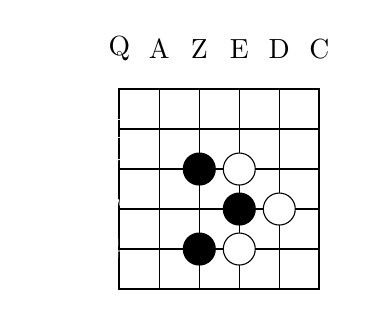
\begin{tikzpicture}[x=0.2in,y=0.2in]
    \draw[step=1] (0,0) grid (5,5);
    \draw[thick] (0,0) rectangle (5,5);
    \draw[fill=black] (2,1) circle (0.4);
    \draw[fill=black] (2,3) circle (0.4);
    \draw[fill=black] (3,2) circle (0.4);
    \draw[fill=white] (3,1) circle (0.4);
    \draw[fill=white] (3,3) circle (0.4);
    \draw[fill=white] (4,2) circle (0.4);
    \node at (-1,0) {\textcolor{white}{\contour{black}{B}}};
    \node at (-1,1) {\textcolor{white}{\contour{black}{G}}};
    \node at (-1,2) {\textcolor{white}{\contour{black}{T}}};
    \node at (-1,3) {\textcolor{white}{\contour{black}{N}}};
    \node at (-1,4) {\textcolor{white}{\contour{black}{H}}};
    \node at (-1,5) {\textcolor{white}{\contour{black}{Y}}};
    \node at (0,6) {Q};
    \node at (1,6) {A};
    \node at (2,6) {Z};
    \node at (3,6) {E};
    \node at (4,6) {D};
    \node at (5,6) {C};
  \end{tikzpicture}
  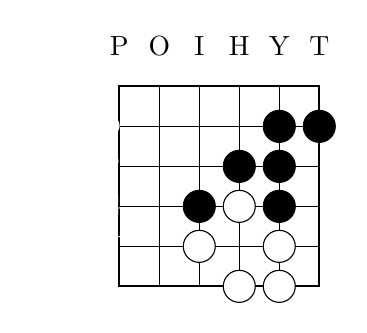
\begin{tikzpicture}[x=0.2in,y=0.2in]
    \draw[step=1] (0,0) grid (5,5);
    \draw[thick] (0,0) rectangle (5,5);
    \draw[fill=black] (2,2) circle (0.4);
    \draw[fill=black] (3,3) circle (0.4);
    \draw[fill=black] (4,2) circle (0.4);
    \draw[fill=black] (4,3) circle (0.4);
    \draw[fill=black] (4,4) circle (0.4);
    \draw[fill=black] (5,4) circle (0.4);
    \draw[fill=white] (2,1) circle (0.4);
    \draw[fill=white] (3,0) circle (0.4);
    \draw[fill=white] (3,2) circle (0.4);
    \draw[fill=white] (4,0) circle (0.4);
    \draw[fill=white] (4,1) circle (0.4);
    \node at (-1,0) {\textcolor{white}{\contour{black}{J}}};
    \node at (-1,1) {\textcolor{white}{\contour{black}{U}}};
    \node at (-1,2) {\textcolor{white}{\contour{black}{G}}};
    \node at (-1,3) {\textcolor{white}{\contour{black}{F}}};
    \node at (-1,4) {\textcolor{white}{\contour{black}{D}}};
    \node at (-1,5) {\textcolor{white}{\contour{black}{S}}};
    \node at (0,6) {P};
    \node at (1,6) {O};
    \node at (2,6) {I};
    \node at (3,6) {H};
    \node at (4,6) {Y};
    \node at (5,6) {T};
  \end{tikzpicture}
  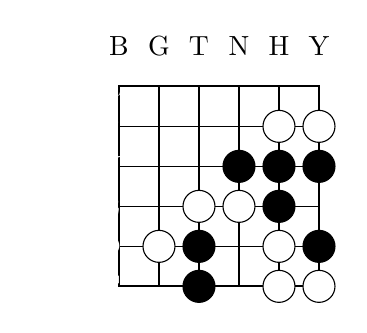
\begin{tikzpicture}[x=0.2in,y=0.2in]
    \draw[step=1] (0,0) grid (5,5);
    \draw[thick] (0,0) rectangle (5,5);
    \draw[fill=white] (1,1) circle (0.4);
    \draw[fill=white] (2,2) circle (0.4);
    \draw[fill=white] (3,2) circle (0.4);
    \draw[fill=white] (4,0) circle (0.4);
    \draw[fill=white] (4,1) circle (0.4);
    \draw[fill=white] (4,4) circle (0.4);
    \draw[fill=white] (5,0) circle (0.4);
    \draw[fill=white] (5,4) circle (0.4);
    \draw[fill=black] (2,0) circle (0.4);
    \draw[fill=black] (2,1) circle (0.4);
    \draw[fill=black] (3,3) circle (0.4);
    \draw[fill=black] (4,2) circle (0.4);
    \draw[fill=black] (4,3) circle (0.4);
    \draw[fill=black] (5,1) circle (0.4);
    \draw[fill=black] (5,3) circle (0.4);
    \node at (-1,0) {\textcolor{white}{\contour{black}{C}}};
    \node at (-1,1) {\textcolor{white}{\contour{black}{D}}};
    \node at (-1,2) {\textcolor{white}{\contour{black}{E}}};
    \node at (-1,3) {\textcolor{white}{\contour{black}{V}}};
    \node at (-1,4) {\textcolor{white}{\contour{black}{F}}};
    \node at (-1,5) {\textcolor{white}{\contour{black}{R}}};
    \node at (0,6) {B};
    \node at (1,6) {G};
    \node at (2,6) {T};
    \node at (3,6) {N};
    \node at (4,6) {H};
    \node at (5,6) {Y};
  \end{tikzpicture}

  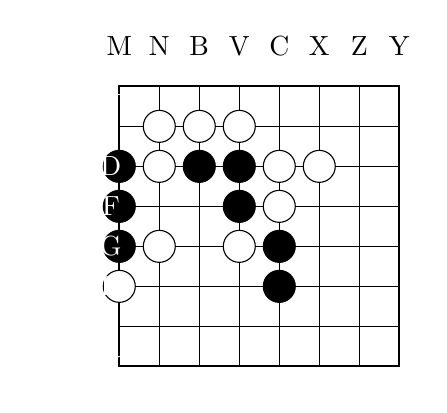
\begin{tikzpicture}[x=0.2in,y=0.2in]
    \draw[step=1] (0,0) grid (7,7);
    \draw[thick] (0,0) rectangle (7,7);
    \draw[fill=white] (0,2) circle (0.4);
    \draw[fill=white] (1,3) circle (0.4);
    \draw[fill=white] (1,5) circle (0.4);
    \draw[fill=white] (1,6) circle (0.4);
    \draw[fill=white] (2,6) circle (0.4);
    \draw[fill=white] (3,3) circle (0.4);
    \draw[fill=white] (3,6) circle (0.4);
    \draw[fill=white] (4,4) circle (0.4);
    \draw[fill=white] (4,5) circle (0.4);
    \draw[fill=white] (5,5) circle (0.4);
    \draw[fill=black] (0,3) circle (0.4);
    \draw[fill=black] (0,4) circle (0.4);
    \draw[fill=black] (0,5) circle (0.4);
    \draw[fill=black] (2,5) circle (0.4);
    \draw[fill=black] (3,4) circle (0.4);
    \draw[fill=black] (3,5) circle (0.4);
    \draw[fill=black] (4,2) circle (0.4);
    \draw[fill=black] (4,3) circle (0.4);
    \node at (-1,0) {\textcolor{white}{\contour{black}{K}}};
    \node at (-1,1) {\textcolor{white}{\contour{black}{J}}};
    \node at (-1,2) {\textcolor{white}{\contour{black}{H}}};
    \node at (-1,3) {\textcolor{white}{\contour{black}{G}}};
    \node at (-1,4) {\textcolor{white}{\contour{black}{F}}};
    \node at (-1,5) {\textcolor{white}{\contour{black}{D}}};
    \node at (-1,6) {\textcolor{white}{\contour{black}{S}}};
    \node at (-1,7) {\textcolor{white}{\contour{black}{A}}};
    \node at (0,8) {M};
    \node at (1,8) {N};
    \node at (2,8) {B};
    \node at (3,8) {V};
    \node at (4,8) {C};
    \node at (5,8) {X};
    \node at (6,8) {Z};
    \node at (7,8) {Y};
  \end{tikzpicture}
  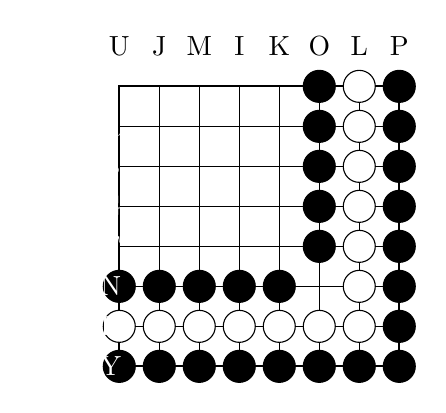
\begin{tikzpicture}[x=0.2in,y=0.2in]
    \draw[step=1] (0,0) grid (7,7);
    \draw[thick] (0,0) rectangle (7,7);
    \foreach \x in {0,1,2,3,4,5,6,7} {
      \draw[fill=black] (\x,0) circle (0.4);
    }
    \foreach \x in {1,2,3,4,5,6,7} {
      \draw[fill=black] (7,\x) circle (0.4);
    }
    \foreach \x in {0,1,2,3,4,5,6} {
      \draw[fill=white] (\x,1) circle (0.4);
    }
    \foreach \x in {2,3,4,5,6,7} {
      \draw[fill=white] (6,\x) circle (0.4);
    }
    \foreach \x in {0,1,2,3,4} {
      \draw[fill=black] (\x,2) circle (0.4);
    }
    \foreach \x in {3,4,5,6,7} {
      \draw[fill=black] (5,\x) circle (0.4);
    }
    \node at (-1,0) {\textcolor{white}{\contour{black}{Y}}};
    \node at (-1,1) {\textcolor{white}{\contour{black}{H}}};
    \node at (-1,2) {\textcolor{white}{\contour{black}{N}}};
    \node at (-1,3) {\textcolor{white}{\contour{black}{T}}};
    \node at (-1,4) {\textcolor{white}{\contour{black}{G}}};
    \node at (-1,5) {\textcolor{white}{\contour{black}{B}}};
    \node at (-1,6) {\textcolor{white}{\contour{black}{R}}};
    \node at (-1,7) {\textcolor{white}{\contour{black}{F}}};
    \node at (0,8) {U};
    \node at (1,8) {J};
    \node at (2,8) {M};
    \node at (3,8) {I};
    \node at (4,8) {K};
    \node at (5,8) {O};
    \node at (6,8) {L};
    \node at (7,8) {P};
  \end{tikzpicture}
  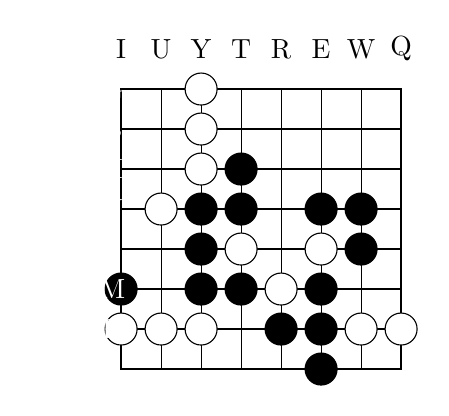
\begin{tikzpicture}[x=0.2in,y=0.2in]
    \draw[step=1] (0,0) grid (7,7);
    \draw[thick] (0,0) rectangle (7,7);
    \draw[fill=black] (0,2) circle (0.4);
    \foreach \x in {2,3,4} {
      \draw[fill=black] (2,\x) circle (0.4);
    }
    \foreach \x in {2,4,5} {
      \draw[fill=black] (3,\x) circle (0.4);
    }
    \draw[fill=black] (4,1) circle (0.4);
    \foreach \x in {0,1,2,4} {
      \draw[fill=black] (5,\x) circle (0.4);
    }
    \foreach \x in {3,4} {
      \draw[fill=black] (6,\x) circle (0.4);
    }
    \foreach \x in {1,4} {
      \draw[fill=white] (1,\x) circle (0.4);
    }
    \foreach \x in {1,5,6,7} {
      \draw[fill=white] (2,\x) circle (0.4);
    }
    \draw[fill=white] (3,3) circle (0.4);
    \draw[fill=white] (4,2) circle (0.4);
    \draw[fill=white] (5,3) circle (0.4);
    \draw[fill=white] (0,1) circle (0.4);
    \draw[fill=white] (6,1) circle (0.4);
    \draw[fill=white] (7,1) circle (0.4);
    \node at (-1,0) {\textcolor{white}{\contour{black}{L}}};
    \node at (-1,1) {\textcolor{white}{\contour{black}{K}}};
    \node at (-1,2) {\textcolor{white}{\contour{black}{M}}};
    \node at (-1,3) {\textcolor{white}{\contour{black}{J}}};
    \node at (-1,4) {\textcolor{white}{\contour{black}{N}}};
    \node at (-1,5) {\textcolor{white}{\contour{black}{H}}};
    \node at (-1,6) {\textcolor{white}{\contour{black}{B}}};
    \node at (-1,7) {\textcolor{white}{\contour{black}{G}}};
    \node at (0,8) {I};
    \node at (1,8) {U};
    \node at (2,8) {Y};
    \node at (3,8) {T};
    \node at (4,8) {R};
    \node at (5,8) {E};
    \node at (6,8) {W};
    \node at (7,8) {Q};
  \end{tikzpicture}

  \begin{tikzpicture}[x=0.2in,y=0.2in]
    \draw[step=1] (0,0) grid (9,9);
    \draw[thick] (0,0) rectangle (9,9);
    \foreach \x in {2,3,4,5,6,7} {
      \draw[fill=white] ($(\x,\x)+(-1,0)$) circle (0.4);
      \draw[fill=white] ($(\x,\x)+(2,0)$) circle (0.4);
    }
    \foreach \x in {2,3,4,5,6,7} {
      \draw[fill=black] (\x,\x) circle (0.4);
      \draw[fill=black] ($(\x,\x)+(1,0)$) circle (0.4);
    }
    \draw[fill=white] (2,1) circle (0.4);
    \draw[fill=white] (7,8) circle (0.4);
    \draw[fill=white] (8,8) circle (0.4);
    \node at (-1,0) {\textcolor{white}{\contour{black}{W}}};
    \node at (-1,1) {\textcolor{white}{\contour{black}{E}}};
    \node at (-1,2) {\textcolor{white}{\contour{black}{R}}};
    \node at (-1,3) {\textcolor{white}{\contour{black}{T}}};
    \node at (-1,4) {\textcolor{white}{\contour{black}{Y}}};
    \node at (-1,5) {\textcolor{white}{\contour{black}{U}}};
    \node at (-1,6) {\textcolor{white}{\contour{black}{I}}};
    \node at (-1,7) {\textcolor{white}{\contour{black}{O}}};
    \node at (-1,8) {\textcolor{white}{\contour{black}{P}}};
    \node at (-1,9) {\textcolor{white}{\contour{black}{L}}};
    \node at (0,10) {K};
    \node at (1,10) {J};
    \node at (2,10) {H};
    \node at (3,10) {G};
    \node at (4,10) {F};
    \node at (5,10) {D};
    \node at (6,10) {S};
    \node at (7,10) {A};
    \node at (8,10) {N};
    \node at (9,10) {M};
  \end{tikzpicture}
  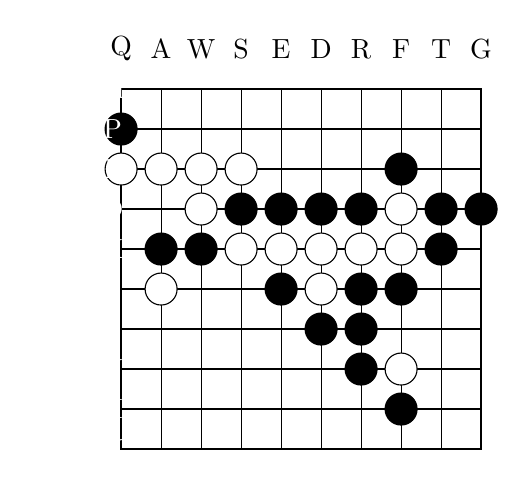
\begin{tikzpicture}[x=0.2in,y=0.2in]
    \draw[step=1] (0,0) grid (9,9);
    \draw[thick] (0,0) rectangle (9,9);
    \draw[fill=black] (0,8) circle (0.4);
    \draw[fill=black] (7,7) circle (0.4);
    \foreach \x in {3,4,5,6,8,9} {
      \draw[fill=black] (\x,6) circle (0.4);
    }
    \foreach \x in {1,2,8} {
      \draw[fill=black] (\x,5) circle (0.4);
    }
    \foreach \x in {4,6,7} {
      \draw[fill=black] (\x,4) circle (0.4);
    }
    \foreach \x in {5,6} {
      \draw[fill=black] (\x,3) circle (0.4);
    }
    \draw[fill=black] (6,2) circle (0.4);
    \draw[fill=black] (7,1) circle (0.4);
    \foreach \x in {0,1,2,3} {
      \draw[fill=white] (\x,7) circle (0.4);
    }
    \foreach \x in {2,7} {
      \draw[fill=white] (\x,6) circle (0.4);
    }
    \foreach \x in {3,4,5,6,7} {
      \draw[fill=white] (\x,5) circle (0.4);
    }
    \foreach \x in {1,5} {
      \draw[fill=white] (\x,4) circle (0.4);
    }
    \draw[fill=white] (7,2) circle (0.4);
    \node at (-1,0) {\textcolor{white}{\contour{black}{Y}}};
    \node at (-1,1) {\textcolor{white}{\contour{black}{H}}};
    \node at (-1,2) {\textcolor{white}{\contour{black}{U}}};
    \node at (-1,3) {\textcolor{white}{\contour{black}{J}}};
    \node at (-1,4) {\textcolor{white}{\contour{black}{I}}};
    \node at (-1,5) {\textcolor{white}{\contour{black}{K}}};
    \node at (-1,6) {\textcolor{white}{\contour{black}{O}}};
    \node at (-1,7) {\textcolor{white}{\contour{black}{L}}};
    \node at (-1,8) {\textcolor{white}{\contour{black}{P}}};
    \node at (-1,9) {\textcolor{white}{\contour{black}{M}}};
    \node at (0,10) {Q};
    \node at (1,10) {A};
    \node at (2,10) {W};
    \node at (3,10) {S};
    \node at (4,10) {E};
    \node at (5,10) {D};
    \node at (6,10) {R};
    \node at (7,10) {F};
    \node at (8,10) {T};
    \node at (9,10) {G};
  \end{tikzpicture}
  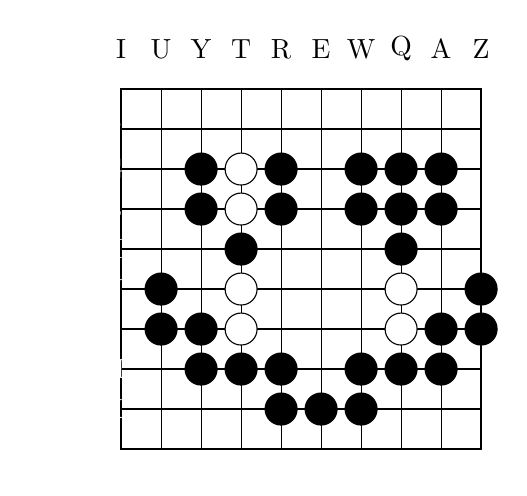
\begin{tikzpicture}[x=0.2in,y=0.2in]
    \draw[step=1] (0,0) grid (9,9);
    \draw[thick] (0,0) rectangle (9,9);
    \foreach \x in {4,5,6} {
      \draw[fill=black] (\x,1) circle (0.4);
    }
    \foreach \x in {2,3,4,6,7,8} {
      \draw[fill=black] (\x,2) circle (0.4);
    }
    \foreach \x in {1,2,8,9} {
      \draw[fill=black] (\x,3) circle (0.4);
    }
    \foreach \x in {1,9} {
      \draw[fill=black] (\x,4) circle (0.4);
    }
    \foreach \x in {3,7} {
      \draw[fill=black] (\x,5) circle (0.4);
    }
    \foreach \x in {2,4,6,7,8} {
      \draw[fill=black] (\x,6) circle (0.4);
      \draw[fill=black] (\x,7) circle (0.4);
    }
    \foreach \x in {3,4,6,7} {
      \draw[fill=white] (3,\x) circle (0.4);
    }
    \foreach \x in {3,4} {
      \draw[fill=white] (7,\x) circle (0.4);
    }
    \node at (-1,0) {\textcolor{white}{\contour{black}{L}}};
    \node at (-1,1) {\textcolor{white}{\contour{black}{K}}};
    \node at (-1,2) {\textcolor{white}{\contour{black}{M}}};
    \node at (-1,3) {\textcolor{white}{\contour{black}{J}}};
    \node at (-1,4) {\textcolor{white}{\contour{black}{N}}};
    \node at (-1,5) {\textcolor{white}{\contour{black}{H}}};
    \node at (-1,6) {\textcolor{white}{\contour{black}{B}}};
    \node at (-1,7) {\textcolor{white}{\contour{black}{G}}};
    \node at (-1,8) {\textcolor{white}{\contour{black}{F}}};
    \node at (-1,9) {\textcolor{white}{\contour{black}{V}}};
    \node at (0,10) {I};
    \node at (1,10) {U};
    \node at (2,10) {Y};
    \node at (3,10) {T};
    \node at (4,10) {R};
    \node at (5,10) {E};
    \node at (6,10) {W};
    \node at (7,10) {Q};
    \node at (8,10) {A};
    \node at (9,10) {Z};
  \end{tikzpicture}
\end{center}

% % To make the cropped boards,
% % Easy way (macOS/*nix/cygwin): open a terminal, cd into assets and type "make"
% % Hard way: Build all of boards#.tex, then in a terminal run pdfcrop on all of
% %           the resulting boards#.pdf files.
% \begin{center}
%   \contournumber{64}
%   \resizebox{6in}{!}{
%   \begin{tikzpicture}
%     \node[anchor=south west,inner sep=0] (image) at
%     (0,0){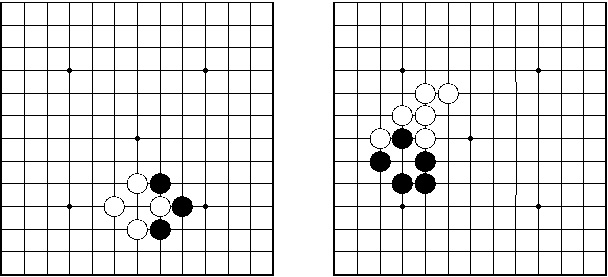
\includegraphics[scale=1.5]{gogetem/assets/boards1-crop}};
%     % left board coordinate system
%     \foreach \x in {0,...,12}
%     \node at (\x * 0.58, 7.3){\contour{black}{\AlphAlph{\x + 14}}};
%     \foreach \x in {0,...,12}
%     \node at (-0.25, \x * 0.58){\contour{black}{\textcolor{white}{\AlphAlph{13 -
%           \x}}}};
%     % right board coordinate system
%   \foreach \x in {0,...,12} \node at (8.5 + \x * 0.58,
%   7.3){\contour{black}{\AlphAlph{\x + 14}}}; \foreach \x in {0,...,12} \node at
%   (8.2, \x * 0.58){\contour{black}{\textcolor{white}{\AlphAlph{13 - \x}}}};
%   \end{tikzpicture}
%   }
%
%   \vfill
%
%   \resizebox{6in}{!}{
%   \begin{tikzpicture}
%     \node[anchor=south west,inner sep=0] (image) at
%     (0,0){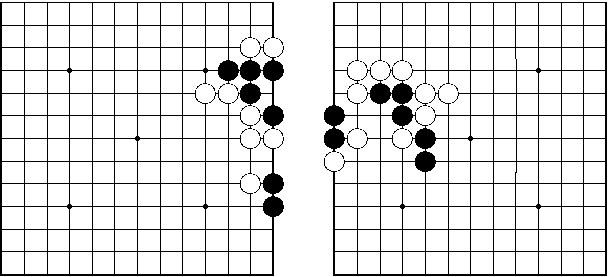
\includegraphics[scale=1.5]{gogetem/assets/boards2-crop}};
%     % left board coordinate system
%     \foreach \x in {0,...,12}
%     \node at (\x * 0.58, 7.3){\contour{black}{\AlphAlph{\x + 14}}};
%     \foreach \x in {0,...,12}
%     \node at (-0.25, \x * 0.58){\contour{black}{\textcolor{white}{\AlphAlph{13 -
%           \x}}}};
%     % right board coordinate system
%     \foreach \x in {0,...,12}
%     \node at (8.5 + \x * 0.58, 7.3){\contour{black}{\AlphAlph{\x + 14}}};
%     \foreach \x in {0,...,12}
%     \node at (8, \x * 0.58){\contour{black}{\textcolor{white}{\AlphAlph{13 - \x}}}};
%   \end{tikzpicture}
%   }
%
%   \vfill
%   \newpage
%
%   \resizebox{6in}{!}{
%   \begin{tikzpicture}
%     \node[anchor=south west,inner sep=0] (image) at
%     (0,0){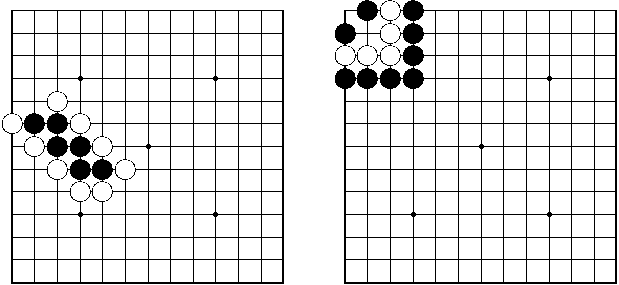
\includegraphics[scale=1.5]{gogetem/assets/boards3-crop}};
%     % left board coordinate system
%     \foreach \x in {0,...,12}
%     \node at (0.35 + \x * 0.58, 7.6){\contour{black}{\AlphAlph{\x + 14}}};
%     \foreach \x in {0,...,12}
%     \node at (-0.25, \x * 0.58){\contour{black}{\textcolor{white}{\AlphAlph{13 -
%           \x}}}};
%     % right board coordinate system
%     \foreach \x in {0,...,12}
%     \node at (8.7 + \x * 0.58, 7.5){\contour{black}{\AlphAlph{\x + 14}}};
%     \foreach \x in {0,...,12}
%     \node at (8.2, \x * 0.58){\contour{black}{\textcolor{white}{\AlphAlph{13 - \x}}}};
%   \end{tikzpicture}
%   }
%
%   \vfill
%
%   \resizebox{6in}{!}{
%   \begin{tikzpicture}
%     \node[anchor=south west,inner sep=0] (image) at
%     (0,0){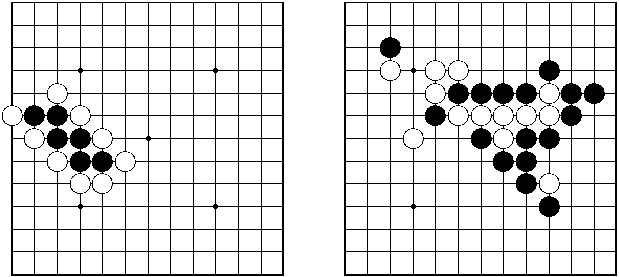
\includegraphics[scale=1.5]{gogetem/assets/boards4-crop}};
%     % left board coordinate system
%     \foreach \x in {0,...,12}
%     \node at (0.3 + \x * 0.58, 7.5){\contour{black}{\AlphAlph{\x + 14}}};
%     \foreach \x in {0,...,12}
%     \node at (-0.25, \x * 0.58){\contour{black}{\textcolor{white}{\AlphAlph{13 -
%           \x}}}};
%     % right board coordinate system
%     \foreach \x in {0,...,12}
%     \node at (8.7 + \x * 0.58, 7.3){\contour{black}{\AlphAlph{\x + 14}}};
%     \foreach \x in {0,...,12}
%     \node at (8.2, \x * 0.58){\contour{black}{\textcolor{white}{\AlphAlph{13 - \x}}}};
%   \end{tikzpicture}
%   }
%
%   \vfill
%
%   \resizebox{3in}{!}{
%   \begin{tikzpicture}
%     \node[anchor=south west,inner sep=0] (image) at
%     (0,0){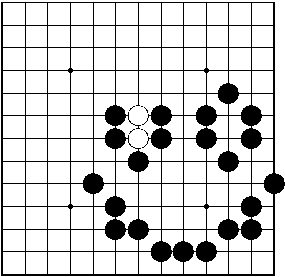
\includegraphics[scale=1.5]{gogetem/assets/boards5-crop}};
%     % left board coordinate system
%     \foreach \x in {0,...,12}
%     \node at (\x * 0.58, 7.3){\contour{black}{\AlphAlph{\x + 14}}};
%     \foreach \x in {0,...,12}
%     \node at (-0.25, \x * 0.58){\contour{black}{\textcolor{white}{\AlphAlph{13 -
%           \x}}}};
%   \end{tikzpicture}
%   }

% \end{center}

% Include below for aucTeX integration
%%% Local Variables:
%%% mode: latex
%%% TeX-master: "../mapp-challenge-18-game-book"
%%% End:
